\documentclass[12pt,a4paper]{article}
\usepackage[utf8]{inputenc}
\usepackage[T5]{fontenc}
\usepackage[vietnamese]{babel}
\usepackage{amsmath, amssymb}
\usepackage{geometry}
\geometry{a4paper, margin=2cm}

% --- Các gói hỗ trợ màu sắc và giao diện ---
\usepackage{xcolor}
\usepackage{titlesec}
\usepackage{graphicx} % Hỗ trợ chèn ảnh
\usepackage{caption}  % Hỗ trợ caption ảnh/bảng
\usepackage{float}    % Hỗ trợ định vị trí ảnh (H)
\usepackage{enumitem} % Tùy chỉnh danh sách (a, b, c, dấu chấm)
\usepackage[skins,breakable]{tcolorbox} % Tạo khung văn bản

% --- Định nghĩa màu sắc ---
\definecolor{darkblue}{RGB}{0, 51, 102}
\definecolor{lightblue}{RGB}{230, 240, 255}

% --- Tùy chỉnh màu sắc và format cho các đề mục ---
\titleformat{\section}
  {\normalfont\Large\bfseries\color{darkblue}}{\thesection.}{1em}{}
\titleformat{\subsection}
  {\normalfont\large\bfseries\color{darkblue}}{\thesubsection.}{1em}{}
\titleformat{\subsubsection}
  {\normalfont\normalsize\bfseries\color{darkblue}}{\thesubsubsection.}{1em}{}

% --- Cấu hình khung mẫu (tcolorbox) ---
\newtcolorbox{infobox}[1][]{
    colback=lightblue,      % Màu nền xanh nhạt
    colframe=darkblue,      % Màu viền xanh đậm
    fonttitle=\bfseries,    % Font tiêu đề in đậm
    title=#1,               % Tiêu đề (tùy chọn)
    arc=4pt,                % Bo góc viền
    boxrule=1pt,            % Độ dày viền
    left=10pt, right=10pt, top=10pt, bottom=10pt % Căn lề trong khung
}

% Tùy chỉnh màu cho link và mục lục
\usepackage[colorlinks=true, linkcolor=black, urlcolor=darkblue, citecolor=darkblue]{hyperref}

\begin{document}
\hypersetup{pageanchor=false}

% =================== TRANG BÌA ===================
\begin{titlepage}
    \centering
    
\includegraphics[width=8.2cm]{logo khoa.png}\\[0cm]
    {\textbf{{TRƯỜNG ĐẠI HỌC KHOA HỌC TỰ NHIÊN, ĐHQG-HCM}}}\\
    {\textbf{\textcolor{black}{KHOA CÔNG NGHỆ THÔNG TIN}}}\\[2.5cm]

    % Đường kẻ trang trí màu xanh đậm
    {\color{darkblue}\rule{\textwidth}{1.5pt}}\\[0.8cm]
    {\Huge \textbf{\textcolor{darkblue}{BÁO CÁO ĐỒ ÁN 1}}}\\[0.5cm]
    {\color{darkblue}\rule{\textwidth}{1.5pt}}\\[1.5cm]
    
    {\Large \textbf{\textcolor{darkblue}{MA TRẬN VÀ CƠ SỞ CỦA TÍNH TOÁN KHOA HỌC}}}\\[3cm]

    
        \large
        \textbf{\textcolor{darkblue}{Giảng viên hướng dẫn:}} \textcolor{black}{ThS. Võ Nam Thục Đoan, ThS. Lê Nhựt Nam}\\[0.5cm]
        \textbf{\textcolor{darkblue}{Nhóm thực hiện:}} \textcolor{black}{Nhóm 14}\\[0.5cm]
        \textbf{\textcolor{darkblue}{Thành viên nhóm:}}\\
        \textcolor{black}{1. Phan Anh Tuấn - 23120187}\\
        \textcolor{black}{2. Nguyễn Thị Diễm Thúy - 24120229}\\
        \textcolor{black}{3. Âu Bảo Trân - 24120468}\\
        \textcolor{black}{4. Huỳnh Trần Phước Thiện - 24120454}\\
   

    \vfill
    {\large \textcolor{black}{TP. Hồ Chí Minh, \today}}
\end{titlepage}

% =================== MỤC LỤC ===================
\newpage
\tableofcontents
\newpage
\hypersetup{pageanchor=true}
% =================== NỘI DUNG CHÍNH ===================

\section{Phần 1: Phép khử Gauss và Các Ứng Dụng}
\subsection{Phép khử Gauss}
Trong phần này, nhóm chúng tôi trình bày các khái niệm nền tảng về đại số tuyến tính phục vụ cho việc cài đặt thuật toán khử Gauss.

\subsubsection{Cơ sở lý thuyết}

\begin{infobox}[Định nghĩa 1.1: Ma trận tăng cường]
Xét hệ phương trình tuyến tính $Ax = b$, ma trận tăng cường $[A | b]$ được ký hiệu là:
\begin{equation}
[A | b] = \begin{pmatrix}
a_{11} & a_{12} & \cdots & a_{1n} & | & b_1 \\
a_{21} & a_{22} & \cdots & a_{2n} & | & b_2 \\
\vdots & \vdots & \ddots & \vdots & | & \vdots \\
a_{m1} & a_{m2} & \cdots & a_{mn} & | & b_m
\end{pmatrix}
\end{equation}
\end{infobox}

\textbf{Lý do sử dụng Partial Pivoting:} Trong tính toán thực tế với số thực, việc chia cho một số cực nhỏ sẽ gây ra sai số lớn (overflow hoặc round-off error). 

\begin{infobox}[Chiến lược chọn phần tử chốt (Partial Pivoting)]
Tại mỗi bước khử, thuật toán xác định dòng $max\_row$ (tính từ dòng hiện tại $r$ đến dòng cuối cùng) có giá trị tuyệt đối tại cột $c$ lớn nhất:
\begin{equation}
|A_{max\_row, c}| = \max_{r \le k < rows} |A_{k, c}|
\end{equation}
Nếu $|A_{max\_row, c}| > \epsilon$ (ngưỡng sai số, với $\epsilon = 10^{-14}$), tiến hành hoán đổi dòng $r$ và dòng $max\_row$ để tối ưu tính ổn định số học và tránh lỗi chia cho $0$.
\end{infobox}

\subsubsection{Phân tích kỹ thuật và cài đặt}
Quy trình thực hiện thuật toán bao gồm hai bước chính:

\begin{enumerate}[label=\textbf{\alph*) Bước \arabic*:}, leftmargin=*, align=left]
\item \textbf{Phép khử Gauss (Gaussian Elimination):}
Duyệt đồng thời chỉ số dòng $r$ và cột $c$ để biến đổi ma trận về dạng bậc thang (REF).
\begin{itemize}[leftmargin=1.5em]
    \item \textbf{Tìm chốt:} Xác định dòng $max\_row$ có phần tử trị tuyệt đối lớn nhất tại cột $c$.
    \item \textbf{Xử lý suy biến:} Nếu $|A_{max\_row, c}| < \epsilon$, bỏ qua cột này và tăng chỉ số $c$ để tìm chốt ở cột tiếp theo.
    \item \textbf{Hoán đổi dòng:} Nếu $max\_row \neq r$, thực hiện hoán đổi dòng $r \leftrightarrow max\_row$ và tăng biến đếm $swaps$.
    \item \textbf{Phép biến đổi dòng:} Với mọi dòng $k > r$, thực hiện triệt tiêu:
    \begin{equation}
    R_k \leftarrow R_k - \left( \frac{A_{k,c}}{A_{r,c}} \right) \cdot R_r, \quad b_k \leftarrow b_k - \left( \frac{A_{k,c}}{A_{r,c}} \right) \cdot b_r
    \end{equation}
\end{itemize}

\item \textbf{Phép thế ngược (Back-substitution):}
Giải hệ phương trình từ dưới lên để tìm vector nghiệm $x$ (hỗ trợ cả trường hợp vô số nghiệm).
\begin{itemize}[leftmargin=1.5em]
    \item \textbf{Thiết lập biến tự do:} Mặc định khởi tạo mỗi biến $x_j$ là một biến tự do có dạng: $x_j = 0 + 1 \cdot t_j$.
    \item \textbf{Xác định biến phụ thuộc:} Với mỗi dòng $i$ có phần tử chốt tại $pivot\_col$:
    \begin{itemize}
        \item \textbf{Kiểm tra vô nghiệm:} Nếu dòng $i$ toàn số $0$ nhưng $b_i \neq 0$, hệ vô nghiệm.
        \item \textbf{Tính tổng đã biết:} $sum\_known = \displaystyle\sum_{j > pivot\_col} U_{ij} x_j$.
        \item \textbf{Cập nhật nghiệm:} Biến tại vị trí chốt được tính theo công thức:
        \begin{equation}
        x_{pivot\_col} = \frac{b_i - sum\_known}{U_{i, pivot\_col}}
        \end{equation}
    \end{itemize}
    \item \textbf{Định dạng đầu ra:} Trả về danh sách các từ điển biểu diễn hằng số và hệ số của các tham số tự do $t_j$.
\end{itemize}
\end{enumerate}

\subsubsection{Kết quả trả về}
\begin{infobox}[Ma trận sau khi khử Gauss]
Ma trận tăng cường $[A | b]$ sau khi khử Gauss sẽ trở thành ma trận tam giác trên $[U | c]$:
\begin{equation}
[U | c] = \begin{pmatrix}
u_{11} & u_{12} & \cdots & u_{1n} & | & c_1 \\
0      & u_{22} & \cdots & u_{2n} & | & c_2 \\
\vdots & \vdots & \ddots & \vdots & | & \vdots \\
0      & 0      & \cdots & u_{mn} & | & c_m
\end{pmatrix}
\end{equation}
\end{infobox}

\subsubsection{Kiểm chứng kết quả bằng thư viện NumPy}
Hàm \texttt{verify\_solution} thực hiện đánh giá nghiệm dựa trên định lý Kronecker-Capelli và các phép toán ma trận của \texttt{NumPy}.

\begin{enumerate}[label=\textbf{\alph*)}, leftmargin=*, align=left]
\item \textbf{Định dạng dữ liệu:} Chuyển đổi ma trận $A$, vector $b$ và nghiệm $my\_x$ (từ dạng từ điển hoặc phân số) về kiểu số thực (\texttt{float}) trong mảng NumPy để xử lý.

\item \textbf{Kiểm tra tính nhất quán:} Sử dụng hàm \texttt{np.linalg.matrix\_rank} để so sánh hạng của ma trận hệ số $\operatorname{rank}(A)$ và hạng của ma trận tăng cường $\operatorname{rank}([A\mid b])$:
\begin{itemize}[leftmargin=*]
    \item Nếu $\operatorname{rank}(A) \ne \operatorname{rank}([A\mid b])$ thì hệ vô nghiệm. Nếu thuật toán tự cài trả về \texttt{None}, kết quả được xem là chính xác.
    \item Nếu $\operatorname{rank}(A) = \operatorname{rank}([A\mid b])$ thì hệ có nghiệm.
\end{itemize}

\item \textbf{Đánh giá sai số:} Sử dụng phép nhân ma trận $A\mathbf{x}$ và so sánh với vector $\mathbf{b}$ thông qua hàm \texttt{np.allclose} với ngưỡng sai số tuyệt đối $\epsilon = 10^{-12}$.

\item \textbf{Kết luận:} Trình bày thông báo \texttt{SUCCESS} nếu kết quả khớp hoàn toàn hoặc \texttt{FAILED} nếu có sự sai lệch.
\end{enumerate}

\begin{infobox}[Tiêu chuẩn kiểm chứng khử Gauss]
Kết quả giải hệ phương trình được đánh giá là chính xác nếu đảm bảo sai số nằm trong ngưỡng cho phép:
\begin{equation}
\lVert A\mathbf{x} - \mathbf{b} \rVert < \epsilon \quad \text{với} \quad \epsilon = 10^{-12}
\end{equation}
\end{infobox}


\subsection{Định thức ma trận}
Dựa trên thuật toán khử Gauss với chiến lược chọn phần tử chốt (Partial Pivoting), định thức của ma trận vuông $A$ được tính toán thông qua việc đưa ma trận về dạng tam giác trên.

\subsubsection{Cơ sở lý thuyết}
\begin{infobox}[Nguyên lý tính định thức]
Giả sử ma trận $A$ được đưa về dạng tam giác trên $U$ sau $s$ lần hoán đổi dòng. Khi đó, định thức của $A$ bằng tích các phần tử trên đường chéo chính của $U$ nhân với $(-1)^s$:
\begin{equation}
\det(A) = (-1)^s \cdot \prod_{i=1}^{n} u_{ii}
\end{equation}
\end{infobox}

\subsubsection{Phân tích kỹ thuật và cài đặt}
Thuật toán cài đặt trong hàm \texttt{determinant(A)} tuân thủ quy trình sau:

\begin{enumerate}[label=\textbf{\alph*) Bước \arabic*:}, leftmargin=*, align=left]
\item \textbf{Kiểm tra điều kiện:} Chương trình xác nhận $A$ là ma trận vuông ($n \times n$). Nếu không thỏa mãn, thuật toán sẽ báo lỗi \texttt{ValueError}.

\item \textbf{Khử Gauss và tính tích đường chéo:}
Duyệt qua từng cột $i$ từ $0$ đến $n-1$:
\begin{itemize}[leftmargin=1.5em]
    \item \textbf{Chọn phần tử trội:} Tìm dòng $max\_row$ có giá trị tuyệt đối tại cột $i$ lớn nhất để làm phần tử chốt (pivot).
    \item \textbf{Hoán đổi dòng:} Nếu $max\_row \neq i$, hoán đổi dòng $i \leftrightarrow max\_row$ và tăng biến đếm số lần hoán đổi $swaps$ lên 1.
    \item \textbf{Cập nhật định thức:} Nhân giá trị \texttt{det} hiện tại với phần tử chốt $A_{i,i}$.
    \item \textbf{Kiểm tra suy biến:} Nếu $|A_{i,i}| < \epsilon $, thuật toán kết luận ma trận suy biến và trả về giá trị $\det(A) = 0$.
\end{itemize}

\item \textbf{Triệt tiêu các phần tử bên dưới:}
Với mỗi dòng $k$ nằm dưới dòng $i$, tính nhân tử $factor = A_{k,i} / A_{i,i}$ và cập nhật dòng $k$ theo quy tắc biến đổi dòng sơ cấp:
\begin{equation}
A_{k} \leftarrow A_{k} - factor \cdot A_{i}
\end{equation}

\item \textbf{Hiệu chỉnh dấu:}
Kết quả cuối cùng được nhân với $(-1)^{swaps}$ để bù lại sự thay đổi dấu mỗi khi có phép hoán đổi dòng xảy ra.
\end{enumerate}

\subsubsection{Kết quả trả về}
\begin{infobox}[Giá trị định thức sau khi khử Gauss]
Nếu thuật toán kết thúc thành công, chương trình trả về một số thực đại diện cho giá trị $\det(A)$. Ngược lại, nếu trong quá trình xử lý xuất hiện phần tử chốt có độ lớn nhỏ hơn ngưỡng $\epsilon$, thuật toán xác nhận ma trận suy biến và lập tức trả về $\det(A) = 0$.
\end{infobox}

\subsubsection{Kiểm chứng kết quả bằng thư viện NumPy}
Việc kiểm chứng định thức giúp xác nhận quá trình khử Gauss và việc theo dõi số lần hoán đổi dòng (biến đổi dấu) được thực hiện đúng đắn. Nhóm sử dụng hàm \texttt{np.linalg.det(A)} của thư viện \texttt{NumPy} làm giá trị tham chiếu.

\begin{enumerate}[label=\textbf{\alph*)}, leftmargin=*, align=left]
    \item \textbf{So sánh:} Sử dụng \texttt{np.isclose} để so sánh giá trị định thức tự tính (\texttt{my\_det}) và giá trị của \texttt{NumPy} (\texttt{np\_det}).
    \item \textbf{Đánh giá sai số:} So sánh độ chênh lệch tuyệt đối giữa hai giá trị dựa trên ngưỡng sai số $\epsilon = 10^{-12}$.
    \item \textbf{Kết luận:} Trình bày thông báo \texttt{SUCCESS} nếu sai số nằm trong giới hạn hoặc \texttt{FAILED} nếu kết quả chênh lệch quá lớn.
\end{enumerate}

\begin{infobox}[Tiêu chuẩn kiểm chứng định thức]
Kết quả tự cài đặt được coi là chính xác và khớp với thư viện chuẩn nếu thỏa mãn:
\begin{equation}
|my\_det - np\_det| \le \epsilon \quad \text{với} \quad \epsilon = 10^{-12}
\end{equation}
\end{infobox}

\subsection{Tìm ma trận nghịch đảo}
Trong mục này, nhóm trình bày cơ sở lý thuyết và quy trình cài đặt thuật toán tìm ma trận nghịch đảo dựa trên phương pháp Gauss-Jordan với ma trận ghép.

\subsubsection{Cơ sở lý thuyết}

\begin{infobox}[Điều kiện tồn tại ma trận nghịch đảo]
Một ma trận vuông $A$ kích thước $n \times n$ là khả nghịch khi và chỉ khi định thức của nó khác $0$, tức là:
\begin{equation}
\det(A) \neq 0
\end{equation}
Khi đó, tồn tại duy nhất một ma trận $A^{-1}$ sao cho:
\begin{equation}
A \cdot A^{-1} = A^{-1} \cdot A = I_n
\end{equation}
trong đó $I_n$ là ma trận đơn vị cấp $n$.
\end{infobox}

Phương pháp trực quan và phổ biến để tìm ma trận nghịch đảo là sử dụng ma trận ghép (Augmented Matrix). Ta ghép ma trận đơn vị $I_n$ vào bên phải ma trận $A$ để thu được ma trận mở rộng:
\begin{equation}
[A \mid I_n]
\end{equation}
Sau đó, áp dụng các phép biến đổi sơ cấp trên dòng theo thuật toán Gauss-Jordan để đưa nửa bên trái từ $A$ về ma trận đơn vị $I_n$. Theo tính chất bảo toàn tương đương dòng, nửa bên phải khi đó sẽ trở thành ma trận nghịch đảo của $A$:
\begin{equation}
[A \mid I_n] \xrightarrow{\text{Biến đổi sơ cấp}} [I_n \mid A^{-1}]
\end{equation}

\subsubsection{Phân tích kỹ thuật và cài đặt}

Hàm \texttt{inverse(A)} được xây dựng để thực thi phương pháp ma trận ghép với độ ổn định số học cao và cơ chế kiểm tra điều kiện đầu vào rõ ràng.

\begin{enumerate}[label=\textbf{\alph*) Bước \arabic*:}, leftmargin=*, align=left]
\item \textbf{Xác thực điều kiện khả nghịch:}
Trước khi bắt đầu biến đổi dòng, thuật toán gọi hàm \texttt{determinant(A)} để kiểm tra tính khả nghịch của ma trận. Nếu:
\begin{equation}
|\det(A)| < \epsilon \quad \text{với} \quad \epsilon = 10^{-12}
\end{equation}
thì ma trận được xem là suy biến và chương trình phát sinh ngoại lệ \texttt{ValueError}.

\item \textbf{Thiết lập ma trận ghép:}
Thuật toán tạo một mảng hai chiều kích thước $n \times 2n$, trong đó:
\begin{itemize}[leftmargin=1.5em]
    \item Nửa bên trái sao chép trực tiếp từ ma trận $A$.
    \item Nửa bên phải là ma trận đơn vị $I_n$ với các phần tử đường chéo bằng $1.0$ và các phần tử còn lại bằng $0.0$.
\end{itemize}
Khi đó ta thu được ma trận mở rộng:
\begin{equation}
\left[A \mid I_n\right]
\end{equation}

\item \textbf{Thực thi Gauss-Jordan với chọn phần tử chốt:}
Với mỗi cột $i$ từ $0$ đến $n-1$, thuật toán thực hiện:
\begin{itemize}[leftmargin=1.5em]
    \item \textbf{Chọn phần tử chốt:} Áp dụng chiến lược Partial Pivoting để tìm dòng $max\_row$ có giá trị tuyệt đối lớn nhất tại cột $i$, sau đó hoán đổi với dòng hiện tại nếu cần.
    \item \textbf{Chuẩn hóa dòng chốt:} Chia toàn bộ dòng thứ $i$ cho giá trị pivot để đưa phần tử chốt về $1$.
    \item \textbf{Khử các phần tử cùng cột:} Với mọi dòng $j \ne i$, thực hiện phép biến đổi dòng:
    \begin{equation}
    R_j \leftarrow R_j - (A_{j,i}) \cdot R_i
    \end{equation}
\end{itemize}
Sau bước này, cột đang xét có dạng của một cột trong ma trận đơn vị.

\item \textbf{Trích xuất kết quả:}
Sau khi hoàn tất $n$ vòng lặp, nửa bên trái của ma trận ghép trở thành ma trận đơn vị $I_n$. Thuật toán lấy các cột từ $n$ đến $2n-1$ để thu được ma trận nghịch đảo:
\begin{equation}
A^{-1} = \left( [I_n \mid A^{-1}] \right)_{[:,\,n:2n]}
\end{equation}
Giá trị này được trả về dưới dạng ma trận hai chiều.
\end{enumerate}

\subsubsection{Kết quả trả về}
\begin{infobox}[Dạng ma trận sau khi hoàn tất Gauss-Jordan]
Nếu thuật toán kết thúc thành công, ma trận ghép ban đầu sẽ được biến đổi về dạng:
\begin{equation}
\left[A \mid I_n\right] \longrightarrow \left[I_n \mid A^{-1}\right]
\end{equation}
Khi đó, khối bên phải chính là ma trận nghịch đảo của $A$. Ngược lại, nếu trong quá trình xử lý xuất hiện pivot có độ lớn quá nhỏ, điều đó xác nhận ma trận không khả nghịch và thuật toán sẽ dừng bằng thông báo lỗi phù hợp.
\end{infobox}

\subsubsection{Kiểm chứng kết quả bằng thư viện NumPy}
Để xác nhận hàm \texttt{inverse(A)} hoạt động chính xác, nhóm đối chiếu kết quả tự cài đặt với các phép toán ma trận của thư viện \texttt{NumPy}.

\begin{enumerate}[label=\textbf{\alph*)}, leftmargin=*, align=left]
    \item \textbf{Định dạng dữ liệu:} Chuyển ma trận đầu vào $A$ và ma trận nghịch đảo tự tính $my\_inv$ về mảng số thực của NumPy.

    \item \textbf{Đối chiếu với kết quả tham chiếu:} Sử dụng hàm \texttt{np.linalg.inv(A)} để thu được ma trận nghịch đảo chuẩn, ký hiệu là \texttt{np\_inv}.

    \item \textbf{Kiểm tra tích ma trận:} Nhân lần lượt $A \cdot my\_inv$ và $my\_inv \cdot A$, sau đó so sánh với ma trận đơn vị $I_n$ bằng \texttt{np.allclose} với ngưỡng sai số $\epsilon = 10^{-12}$.

    \item \textbf{So sánh trực tiếp từng phần tử:} Dùng \texttt{np.allclose(my\_inv, np\_inv)} để kiểm tra ma trận nghịch đảo tự tính có khớp với kết quả tham chiếu của NumPy hay không.

    \item \textbf{Kết luận:} Nếu cả hai phép kiểm tra đều đạt, chương trình trả về thông báo \texttt{SUCCESS}; ngược lại, kết quả được đánh dấu là \texttt{FAILED}.
\end{enumerate}

\begin{infobox}[Tiêu chuẩn kiểm chứng ma trận nghịch đảo]
Kết quả được xem là đúng nếu ma trận nghịch đảo tự tính thỏa:
\begin{equation}
A \cdot A^{-1} \approx I_n \quad \text{và} \quad A^{-1} \cdot A \approx I_n
\end{equation}
\end{infobox}

\subsection{Tìm hạng và cơ sở của các không gian ma trận}
Trong mục này, nhóm trình bày cách xác định hạng của ma trận và xây dựng cơ sở cho các không gian dòng, không gian cột và không gian nghiệm thông qua dạng bậc thang rút gọn (RREF).

\subsubsection{Cơ sở lý thuyết}
Trong đại số tuyến tính, các đặc trưng quan trọng của ma trận $A$ kích thước $m \times n$ có thể được xác định bằng cách đưa ma trận về dạng bậc thang rút gọn (Reduced Row Echelon Form -- RREF) bằng thuật toán Gauss-Jordan.

\begin{infobox}[Định nghĩa dạng bậc thang rút gọn (RREF)]
Ma trận ở dạng RREF khi thỏa mãn ba điều kiện sau:
\begin{enumerate}[label=\textbf{\arabic*)}, leftmargin=*, align=left]
    \item Phần tử cơ sở (pivot) của mỗi dòng khác không phải bằng $1$.
    \item Pivot của dòng dưới nằm về bên phải pivot của dòng trên.
    \item Mọi phần tử khác nằm trong cùng cột với pivot đều bằng $0$.
\end{enumerate}
\end{infobox}

Từ ma trận RREF, ta rút ra các kết luận lý thuyết quan trọng sau:
\begin{itemize}[leftmargin=1.5em]
    \item \textbf{Hạng của ma trận (Rank):} Bằng số lượng pivot trong RREF, hay tương đương với số dòng khác không:
    \begin{equation}
    \operatorname{rank}(A) = \text{số lượng pivot}
    \end{equation}

    \item \textbf{Cơ sở không gian dòng (Row Space Basis):} Là tập hợp các dòng khác không được lấy trực tiếp từ ma trận RREF.

    \item \textbf{Cơ sở không gian cột (Column Space Basis):} Nếu các cột chứa pivot trong RREF có chỉ số là $j_1, j_2, \dots, j_k$, thì cơ sở không gian cột là các cột tương ứng $j_1, j_2, \dots, j_k$ được lấy từ ma trận gốc $A$.

    \item \textbf{Cơ sở không gian nghiệm (Null Space Basis):} Được xác định từ nghiệm của hệ thuần nhất $Ax = 0$. Số vector cơ sở bằng số biến tự do:
    \begin{equation}
    \dim(\mathcal{N}(A)) = n - \operatorname{rank}(A)
    \end{equation}
\end{itemize}

\subsubsection{Phân tích kỹ thuật và cài đặt}
Hàm \texttt{rank\_and\_basis(A)} được cài đặt theo hướng bám sát lý thuyết RREF, đồng thời có bổ sung cơ chế kiểm soát sai số số thực.

\begin{enumerate}[label=\textbf{\alph*) Bước \arabic*:}, leftmargin=*, align=left]
\item \textbf{Khử Gauss-Jordan với Partial Pivoting:}
Với mỗi cột $j$, thuật toán tìm phần tử có giá trị tuyệt đối lớn nhất từ dòng hiện tại trở xuống để chọn làm pivot, sau đó hoán đổi lên dòng đang xét. Cách làm này giúp tránh chia cho số quá nhỏ và tăng độ ổn định số học.

\item \textbf{Xử lý sai số dấu phẩy động:}
Thuật toán sử dụng các ngưỡng sai số để lọc nhiễu số học:
\begin{itemize}[leftmargin=1.5em]
    \item Nếu $\max(|A_{i,j}|) < 10^{-7}$ thì cột đang xét được bỏ qua.
    \item Trong quá trình khử, nếu $|A_{i,k}| < 10^{-9}$ thì phần tử đó được ép về $0.0$.
\end{itemize}
Nhờ đó, ma trận RREF thu được có dạng rõ ràng và dễ trích xuất thông tin.

\item \textbf{Xác định hạng và cơ sở không gian dòng, cột:}
Sau khi ma trận đã ở dạng RREF, thuật toán ghi nhận các cột chứa pivot để suy ra hạng. Từ đó:
\begin{itemize}[leftmargin=1.5em]
    \item Các dòng khác không của RREF tạo thành cơ sở của không gian dòng.
    \item Các cột pivot tương ứng trong ma trận gốc $A$ tạo thành cơ sở của không gian cột.
\end{itemize}

\item \textbf{Trích xuất cơ sở không gian nghiệm:}
Thuật toán xác định danh sách các biến tự do. Với mỗi biến tự do $x_f$, một vector cơ sở được tạo bằng cách đặt $x_f = 1$, các biến tự do còn lại bằng $0$, rồi tính ngược các biến pivot theo quan hệ:
\begin{equation}
x_p = -RREF[r,f]
\end{equation}
trong đó $p$ là chỉ số cột pivot và $r$ là dòng chứa pivot tương ứng.
\end{enumerate}

\subsubsection{Kết quả trả về}
\begin{infobox}[Ý nghĩa của các đại lượng đầu ra]
Hàm \texttt{rank\_and\_basis(A)} trả về các thông tin chính sau:
\begin{itemize}[leftmargin=1.5em]
    \item \textbf{rank:} Hạng của ma trận $A$.
    \item \textbf{row\_basis:} Danh sách các dòng khác không của RREF.
    \item \textbf{col\_basis:} Danh sách các cột pivot được trích từ ma trận gốc $A$.
    \item \textbf{null\_basis:} Danh sách các vector cơ sở của không gian nghiệm $Ax = 0$.
\end{itemize}
Các kết quả này cho phép mô tả đầy đủ cấu trúc tuyến tính của ma trận dưới góc nhìn đại số tuyến tính và tính toán khoa học.
\end{infobox}

\subsubsection{Kiểm chứng kết quả bằng thư viện NumPy}
Để đảm bảo kết quả tự cài đặt là chính xác, nhóm đối chiếu hạng và các không gian cơ sở với các phép toán chuẩn của thư viện \texttt{NumPy}.

\begin{enumerate}[label=\textbf{\alph*)}, leftmargin=*, align=left]
    \item \textbf{Kiểm chứng hạng:} Sử dụng hàm \texttt{np.linalg.matrix\_rank(A)} để so sánh với giá trị \texttt{rank} do thuật toán tự cài trả về.

    \item \textbf{Kiểm chứng không gian cột và không gian dòng:} Kiểm tra tính độc lập tuyến tính và số lượng vector cơ sở thu được. Một tập vector được xem là hợp lệ nếu số vector đúng bằng hạng của ma trận và các vector đó độc lập tuyến tính.

    \item \textbf{Kiểm chứng không gian nghiệm:} Với mỗi vector $v$ trong \texttt{null\_basis}, tính tích ma trận $Av$ và kiểm tra bằng \texttt{np.allclose} rằng $Av \approx 0$. Ngoài ra, số lượng vector trong cơ sở không gian nghiệm phải thỏa công thức chiều.

    \item \textbf{Kết luận:} Nếu tất cả phép kiểm tra đều thỏa mãn, chương trình kết luận \texttt{SUCCESS}; ngược lại, kết quả được đánh dấu là \texttt{FAILED}.
\end{enumerate}

\begin{infobox}[Tiêu chuẩn kiểm chứng không gian nghiệm]
Đối với mỗi vector $v$ trong cơ sở không gian nghiệm, thuật toán kiểm tra:
\begin{equation}
A v \approx 0
\end{equation}
Đồng thời, số lượng vector cơ sở phải thỏa: 
\begin{equation}
\text{len(null\_basis)} = n - \operatorname{rank}(A)
\end{equation}
\end{infobox}

\newpage


\section{Phần 2: Phân Rã Ma Trận và Trực Quan Hóa với Manim}

\subsection{Chéo hóa ma trận (Diagonalizable Matrix)}

Phần này trình bày phương pháp cài đặt thuật toán chéo hóa ma trận vuông $A$ thành dạng $A = PDP^{-1}$, trong đó $P$ là ma trận các vector riêng và $D$ là ma trận đường chéo chứa các trị riêng tương ứng.

\subsubsection{Cơ sở lý thuyết}

Quá trình chéo hóa ma trận là việc tìm kiếm một dạng biểu diễn đơn giản hơn của ma trận vuông thông qua phép biến đổi đồng dạng.

\begin{infobox}[Định nghĩa Ma trận chéo hóa được]
    Một ma trận vuông $A$ cấp $n$ được gọi là \textbf{chéo hóa được} (diagonalizable) nếu tồn tại một ma trận khả nghịch $P$ cấp $n$ và một ma trận đường chéo $D$ sao cho:
    \begin{equation}
        A = PDP^{-1} \quad \text{hay} \quad D = P^{-1}AP
    \end{equation}
    Trong đó:
    \begin{itemize}
        \item Các phần tử trên đường chéo chính của $D$ là các trị riêng $\lambda_1, \lambda_2, \dots, \lambda_n$ của $A$.
        \item Các cột của ma trận $P$ là các vector riêng tương ứng với các trị riêng đó.
    \end{itemize}
\end{infobox}

\textbf{Điều kiện chéo hóa:}
Để một ma trận $A$ cấp $n$ có thể chéo hóa được, các điều kiện sau phải được thỏa mãn:
\begin{enumerate}[label=\textbf{\alph*)}]
    \item \textbf{Số lượng vector riêng:} Ma trận $A$ phải có đủ $n$ vector riêng độc lập tuyến tính. 
    \item \textbf{Bội đại số và Bội hình học:} Với mỗi trị riêng $\lambda_i$, bội hình học (số chiều của không gian nghiệm của hệ $(A - \lambda_i I)v = 0$) phải bằng bội đại số (số lần xuất hiện của trị riêng đó trong phương trình đặc trưng).
    \item \textbf{Trường hợp đủ:} Nếu $A$ có $n$ trị riêng phân biệt thì $A$ chắc chắn chéo hóa được.
\end{enumerate}

\textbf{Ý nghĩa trong tính toán khoa học:}
Việc đưa ma trận về dạng đường chéo giúp tối ưu hóa đáng kể chi phí tính toán, đặc biệt là phép tính lũy thừa ma trận:
\begin{equation}
    A^k = (PDP^{-1})^k = PD^kP^{-1}
\end{equation}
Thay vì thực hiện nhân ma trận $k$ lần với độ phức tạp $O(n^3 \log k)$, ta chỉ cần tính lũy thừa các phần tử trên đường chéo của $D$ với độ phức tạp $O(n)$, sau đó thực hiện hai phép nhân ma trận cố định.

\subsubsection{Cấu trúc mã nguồn và Các hàm xử lý}
Để đảm bảo tính module hóa và dễ dàng kiểm soát sai số tính toán, nhóm đã chia quy trình chéo hóa thành các tập tin bổ trợ trong thư mục \texttt{part2/}:

\begin{enumerate}[label=\textbf{\alph*)}]
    \item \textbf{Tìm trị riêng (File \texttt{eigenvalues\_utils.py}):} 
    Sử dụng thuật toán QR lặp để tìm các trị riêng mà không cần giải phương trình đặc trưng.
    \begin{itemize}
        \item \textbf{Hàm \texttt{qr\_decomposition(A)}:} Thực hiện phân rã trực giao ma trận $A$ thành $Q$ (ma trận trực chuẩn) và $R$ (ma trận tam giác trên) bằng thuật toán Gram-Schmidt.
        \item \textbf{Hàm \texttt{get\_eigenvalues(A)}:} Thực hiện vòng lặp $A_{k+1} = R_k Q_k$. Sau số lần lặp xác định (mặc định 500), các phần tử trên đường chéo của $A_k$ sẽ hội tụ về các trị riêng của ma trận gốc.
    \end{itemize}

    \item \textbf{Tìm vector riêng (File \texttt{eigenvector\_utils.py}):}
    Với mỗi trị riêng $\lambda$ tìm được, nhóm tiến hành giải hệ phương trình thuần nhất $(A - \lambda I)v = 0$.
    \begin{itemize}
        \item \textbf{Hàm \texttt{find\_eigenvectors\_for\_lambda(A, lam)}:} Gọi hàm \texttt{rank\_and\_basis} (từ Phần 1) để tìm cơ sở cho không gian nghiệm (null space).
        \item \textbf{Xử lý ổn định số học:} Nhóm sử dụng hàm \texttt{group\_close\_eigenvalues} để xử lý các trị riêng gần nhau và \texttt{retry\_extract\_null\_space} kết hợp với danh sách \texttt{ROUNDING\_PRECISIONS} để thử lại việc tìm vector riêng với các mức làm tròn khác nhau khi gặp sai số dấu phẩy động.
    \end{itemize}

    \item \textbf{Thực thi chéo hóa (File \texttt{diagonalization.py}):}
    \begin{itemize}
        \item \textbf{Hàm \texttt{diagonalize(A)}:} Hàm điều phối chính, nhận các vector riêng và trị riêng để xây dựng ma trận $P$ và $D$. Hàm cũng kiểm tra điều kiện $len(vectors) < n$ để xác định ma trận có chéo hóa được hay không.
        \item \textbf{Hàm \texttt{construct\_diagonal\_matrix(eigenvals)}:} Tạo ma trận đường chéo $D$ từ danh sách trị riêng đã được chuẩn hóa.
    \end{itemize}
\end{enumerate}

\subsubsection{Thực nghiệm và Đánh giá (Test Suite)}
Nhóm đã xây dựng bộ kiểm thử tự động trong hàm \texttt{diagonalization\_test} để đánh giá độ chính xác thông qua sai số tái cấu trúc (Reconstruction Error):
$$\epsilon = ||A - PDP^{-1}||_F$$

\begin{infobox}[Kết quả kiểm thử tiêu biểu]
    Dựa trên kết quả thực thi, thuật toán đạt độ chính xác rất cao:
    \begin{itemize}
        \item \textbf{Symmetric Matrix 3x3:} Sai số $\approx 4.36 \times 10^{-9}$.
        \item \textbf{Lower Triangular Matrix 3x3:} Sai số $\approx 6.66 \times 10^{-16}$.
        \item \textbf{Repeated Eigenvalues Matrix:} Hệ thống báo lỗi \texttt{Insufficient eigenvectors (Found 1/3)}, phản ánh đúng lý thuyết toán học về ma trận không thể chéo hóa.
    \end{itemize}
\end{infobox}


\subsection{Phân rã Cholesky}
Trong mục này, nhóm trình bày phương pháp phân rã Cholesky dành cho lớp ma trận đối xứng xác định dương, một kỹ thuật quan trọng trong giải hệ tuyến tính, tối ưu hóa số, ước lượng thống kê và mô phỏng ngẫu nhiên. So với các phương pháp phân rã tổng quát, Cholesky khai thác trực tiếp tính đối xứng của ma trận để giảm số phép tính, đồng thời duy trì độ ổn định số học tốt trong nhiều bài toán thực tế.

\subsubsection{Cơ sở lý thuyết}

\begin{infobox}[Định nghĩa 2.2: Phân rã Cholesky]
Cho ma trận đối xứng xác định dương $A \in \mathbb{R}^{n \times n}$. Khi đó tồn tại duy nhất một ma trận tam giác dưới $L$ có các phần tử trên đường chéo chính dương \cite{ref4,ref5} sao cho:
\begin{equation}
A = L L^T
\end{equation}
\end{infobox}

\noindent Sở dĩ phân rã này có ý nghĩa lớn trong tính toán khoa học là vì một ma trận đối xứng xác định dương xuất hiện rất thường xuyên trong các bài toán thực tế, chẳng hạn ma trận hiệp phương sai, ma trận Hessian của bài toán tối ưu lồi hoặc các hệ thu được từ phương pháp bình phương tối thiểu\cite{ref3}. Khi đưa được ma trận về dạng $LL^T$, bài toán ban đầu được rút gọn thành hai hệ tam giác dễ giải hơn nhiều.

\subsubsection{Điều kiện áp dụng và ưu điểm}

\begin{enumerate}[label=\textbf{\alph*)}, leftmargin=*, align=left]
    \item \textbf{Đối xứng:} Ma trận phải thỏa mãn $A = A^T$.

    \item \textbf{Xác định dương:} Với mọi vector khác không $\mathbf{x}$, ta có:
    \begin{equation}
    \mathbf{x}^T A \mathbf{x} > 0
    \end{equation}

    \item \textbf{Hiệu quả tính toán:} So với phép khử Gauss tổng quát hoặc phân rã LU không chuyên biệt, Cholesky tận dụng tính đối xứng để giảm số phép toán và giảm chi phí lưu trữ, đặc biệt hiệu quả khi kích thước ma trận lớn.

    \item \textbf{Ứng dụng rộng rãi:} Phân rã này xuất hiện trong giải hệ tuyến tính $A\mathbf{x}=\mathbf{b}$, hồi quy bình phương tối thiểu, lọc Kalman, Gaussian Process, mô phỏng phân phối chuẩn đa biến và các bài toán tối ưu bậc hai\cite{ref3}.
\end{enumerate}

\subsubsection{Công thức xây dựng ma trận tam giác dưới}

\begin{infobox}[Công thức tính các phần tử của $L$]
Với $A = (a_{ij})$ và $L = (\ell_{ij})$, các phần tử của $L$ được xác định tuần tự theo công thức:
\begin{equation}
\ell_{ii} = \sqrt{a_{ii} - \sum_{k=1}^{i-1} \ell_{ik}^2}
\end{equation}
và với $j < i$:
\begin{equation}
\ell_{ij} = \frac{1}{\ell_{jj}}\left(a_{ij} - \sum_{k=1}^{j-1} \ell_{ik}\ell_{jk}\right)
\end{equation}
Trong khi đó, mọi phần tử phía trên đường chéo chính đều bằng $0$.
\end{infobox}

\noindent\textbf{Nhận xét:}  
Các công thức trên mang tính truy hồi, nghĩa là mỗi phần tử của $L$ chỉ phụ thuộc vào các phần tử đã được tính trước đó. Nhờ vậy, thuật toán có thể triển khai tuần tự theo từng dòng mà không cần thực hiện phép biến đổi toàn cục trên ma trận như phương pháp khử Gauss.


\subsubsection{Phân tích kỹ thuật và cài đặt}

Thuật toán phân rã Cholesky trong chương trình được tổ chức theo hướng kiểm tra điều kiện đầu vào trước, sau đó tính tuần tự từng phần tử của ma trận tam giác dưới $L$. Cách cài đặt này bám sát công thức truy hồi, đồng thời cho phép phát hiện sớm các trường hợp không phù hợp để tránh lan truyền sai số trong toàn bộ quá trình tính toán.

\begin{enumerate}[label=\textbf{\alph*) Bước \arabic*:}, leftmargin=*, align=left]

\item \textbf{Xác thực cấu trúc của ma trận đầu vào:}
Thuật toán trước hết kiểm tra ma trận $A$ có phải là ma trận vuông hay không. Đây là điều kiện bắt buộc vì phân rã Cholesky chỉ được định nghĩa cho ma trận vuông. Nếu số dòng và số cột không khớp, quá trình sẽ dừng ngay với thông báo lỗi phù hợp.

\item \textbf{Kiểm tra tính đối xứng:}
Sau khi bảo đảm ma trận là vuông, chương trình so sánh các phần tử đối xứng qua đường chéo chính để xác nhận $A = A^T$. Trong môi trường tính toán số, phép so sánh được thực hiện cùng với một ngưỡng sai số nhỏ $10^{-9}$ nhằm tránh kết luận sai do sai số dấu phẩy động.

\item \textbf{Khởi tạo ma trận tam giác dưới:}
Thuật toán tạo một ma trận $L$ cùng kích thước với $A$, ban đầu chứa toàn số $0$. Trong suốt quá trình tính toán, chỉ các phần tử trên và dưới đường chéo chính thuộc tam giác dưới mới được cập nhật, còn các phần tử phía trên luôn giữ nguyên bằng $0$.

\item \textbf{Tính phần tử đường chéo chính:}
Với mỗi chỉ số $i$, phần tử $\ell_{ii}$ được xác định bằng căn bậc hai của phần còn lại sau khi trừ đi tổng bình phương các phần tử đã biết trên cùng dòng:
\begin{equation}
\ell_{ii} = \sqrt{a_{ii} - \sum_{k=1}^{i-1} \ell_{ik}^2}
\end{equation}
Đây là bước quan trọng của thuật toán vì biểu thức dưới dấu căn phải dương. Nếu giá trị này không dương, chương trình kết luận ma trận không xác định dương và dừng lại.

\item \textbf{Tính các phần tử dưới đường chéo:}
Sau khi xác định được phần tử chéo $\ell_{jj}$, thuật toán tiếp tục tính các phần tử $\ell_{ij}$ với $i > j$ theo công thức:
\begin{equation}
\ell_{ij} = \frac{1}{\ell_{jj}}\left(a_{ij} - \sum_{k=1}^{j-1} \ell_{ik}\ell_{jk}\right)
\end{equation}
Nhờ cấu trúc truy hồi này, mỗi giá trị mới chỉ phụ thuộc vào các phần tử đã được xác định trước đó, nên quy trình có thể triển khai tuần tự theo từng cột hoặc từng dòng.

\item \textbf{Xử lý sai số số thực:}
Trong quá trình kiểm tra tính đối xứng, chương trình sử dụng một ngưỡng sai số nhỏ ($10^{-9}$) để tránh ảnh hưởng của sai số dấu phẩy động khi so sánh các phần tử.

\item \textbf{Tổ chức đầu ra của thuật toán:}
Nếu quá trình hoàn tất thành công, chương trình trả về ma trận tam giác dưới $L$. Từ đây, các bước tiếp theo như giải hệ tuyến tính, kiểm chứng lại $A \approx LL^T$ hoặc đối chiếu với thư viện chuẩn đều có thể được thực hiện một cách trực tiếp và rõ ràng.

\end{enumerate}

\subsubsection{Ý nghĩa của kết quả trả về}

\begin{infobox}[Kết quả của phân rã Cholesky]
Nếu ma trận đầu vào thỏa điều kiện đối xứng xác định dương, thuật toán trả về ma trận tam giác dưới $L$ sao cho:
\begin{equation}
A = LL^T
\end{equation}
Kết quả này cho phép thay thế bài toán ma trận ban đầu bằng hai bài toán tam giác đơn giản hơn. Ngược lại, nếu một trong các điều kiện đầu vào không thỏa mãn, chương trình sẽ dừng và trả về thông báo lỗi tương ứng thay vì cố tiếp tục tính toán.
\end{infobox}


\begin{figure}[H]
\centering

\[
A =
\begin{pmatrix}
4 & 2 & 2 \\
2 & 5 & 1 \\
2 & 1 & 3
\end{pmatrix}
\quad \longrightarrow \quad
L =
\begin{pmatrix}
2 & 0 & 0 \\
1 & 2 & 0 \\
1 & 0 & \sqrt{2}
\end{pmatrix}
\]

\caption{Minh họa đầu vào và đầu ra của hàm \texttt{cholesky(A)} với ma trận đối xứng xác định dương}
\end{figure}

\subsubsection{Kiểm chứng kết quả bằng thư viện NumPy}

Để xác nhận kết quả phân rã Cholesky là chính xác, nhóm tiến hành kiểm chứng theo nhiều lớp, kết hợp giữa tái tạo ma trận ban đầu và so sánh với các phép toán chuẩn trong \texttt{NumPy}.

\begin{enumerate}[label=\textbf{\alph*)}, leftmargin=*, align=left]
    \item \textbf{Kiểm tra phép tái tạo ma trận:} Sau khi thu được ma trận $L$, chương trình tính lại tích:
    \begin{equation}
    LL^T
    \end{equation}
    rồi so sánh với ma trận đầu vào $A$ bằng \texttt{np.allclose}. Nếu hai ma trận khớp nhau trong sai số cho phép, quá trình phân rã được xem là hợp lệ.\cite{ref6}

    \item \textbf{Kiểm tra cấu trúc tam giác dưới:} Thuật toán xác nhận các phần tử phía trên đường chéo chính của $L$ bằng $0$ hoặc đủ nhỏ để xem như $0$ trong ngưỡng sai số số học.

    \item \textbf{Đối chiếu điều kiện đầu vào:} Với các bộ kiểm thử không đối xứng, không vuông hoặc không xác định dương, chương trình phải trả về lỗi đúng như kỳ vọng. Đây là bước quan trọng để khẳng định phần kiểm tra điều kiện đầu vào hoạt động chính xác.

    \item \textbf{Khả năng mở rộng:}
Trong các ứng dụng nâng cao, kết quả phân rã có thể được sử dụng để giải hệ tuyến tính thông qua hai bước thế tiến và thế lùi.

    \item \textbf{Kết luận:} Khi cả phép tái tạo ma trận, cấu trúc tam giác dưới và các ca kiểm thử biên đều đạt yêu cầu, chương trình kết luận \texttt{True}; ngược lại, kết quả được đánh dấu là \texttt{False}.
\end{enumerate}

\subsubsection{Ứng dụng giải hệ phương trình tuyến tính}
Sau khi phân rã được $A = LL^T$, hệ tuyến tính:
\begin{equation}
A\mathbf{x} = \mathbf{y}
\end{equation}
có thể được viết lại thành hai hệ tam giác đơn giản hơn:
\begin{equation}
L\mathbf{z} = \mathbf{y}, \quad L^T\mathbf{x} = \mathbf{z}
\end{equation}
Khi đó, bài toán ban đầu được giải bằng hai lần thế tiến và thế lùi, giúp giảm chi phí tính toán đáng kể so với việc nghịch đảo ma trận trực tiếp. Về mặt số học, cách tiếp cận này cũng ổn định hơn vì tránh việc tính $A^{-1}$ một cách tường minh, vốn thường không cần thiết và dễ khuếch đại sai số làm tròn.


\subsection{Trực Quan Hóa với Manim}
Bên cạnh việc trình bày công thức và thuật toán, nhóm sử dụng công cụ \texttt{Manim} để trực quan hóa các phép biến đổi ma trận, từ đó giúp người xem dễ hình dung hơn về ý nghĩa hình học và quy trình tính toán. Video demo được tải lên YouTube tại địa chỉ: \url{https://www.youtube.com/watch?v=yl8IB69U9t4}.

\subsubsection{Giới thiệu ngắn về Manim}

\begin{infobox}[Manim là gì?]
\texttt{Manim} (Mathematical Animation Engine) là thư viện chuyên dùng để tạo hoạt ảnh toán học bằng mã lệnh. Công cụ này đặc biệt phù hợp để biểu diễn vector, ma trận, phép biến đổi tuyến tính, không gian riêng và các bước biến đổi thuật toán một cách trực quan, chính xác và có tính thẩm mỹ cao.\cite{ref7}
\end{infobox}

\noindent Việc sử dụng Manim không thay thế phần chứng minh hay phân tích lý thuyết, nhưng đóng vai trò hỗ trợ mạnh trong khâu diễn giải. Đối với các chủ đề như chéo hóa hoặc phân rã ma trận, hình ảnh động giúp người học kết nối công thức đại số với trực giác hình học.

\subsubsection{Các nội dung phù hợp để trực quan hóa}

\begin{enumerate}[label=\textbf{\alph*)}, leftmargin=*, align=left]
    \item \textbf{Biến đổi tác động lên vector:} Minh họa cách ma trận $A$ biến đổi một vector hoặc một lưới tọa độ trong mặt phẳng.

    \item \textbf{Ý nghĩa của vector riêng:} Cho thấy những vector chỉ bị co giãn theo phương cũ sau khi qua phép biến đổi tuyến tính.

    \item \textbf{Quá trình chéo hóa:} Tách ma trận thành chuỗi thao tác $P$, $D$, $P^{-1}$ để giải thích vai trò của cơ sở riêng.

    \item \textbf{Phân rã Cholesky:} Minh họa việc thay một ma trận đối xứng xác định dương bằng tích của ma trận tam giác dưới và chuyển vị của nó.
\end{enumerate}

\subsubsection{Quy trình xây dựng hoạt cảnh}
Trong đồ án, phần trực quan hóa với \texttt{Manim} được xây dựng theo hướng bám sát nội dung toán học đã trình bày ở các mục trước. Mục tiêu của phần này không chỉ là minh họa kết quả cuối cùng, mà còn hỗ trợ người xem theo dõi rõ hơn tiến trình suy luận, từ điều kiện áp dụng, công thức trung gian cho đến kết quả của từng phương pháp. Trên cơ sở đó, nội dung trực quan hóa được tổ chức theo trình tự sau:


\begin{enumerate}[label=\textbf{\alph*) Bước \arabic*:}, leftmargin=*, align=left]

\item \textbf{Giới thiệu bài toán}

Phần mở đầu được dùng để định hướng nội dung cho người xem, trong đó nêu rõ chủ đề chính là phân rã ma trận và chéo hóa ma trận. Việc giới thiệu bài toán ngay từ đầu giúp người xem xác định được phạm vi kiến thức đang được trình bày, đồng thời tạo sự liên kết giữa phần lý thuyết trong báo cáo và phần trực quan hóa bằng \texttt{Manim}.

\item \textbf{Trình bày điều kiện ma trận SPD}

Đối với phân rã Cholesky, trước hết cần làm rõ điều kiện để thuật toán có thể áp dụng, đó là ma trận phải đối xứng xác định dương. Trong phần minh họa, một ma trận cụ thể $A$ được đưa ra để người xem quan sát trực tiếp cấu trúc của ma trận. Từ đó, các đặc trưng quan trọng của ma trận đối xứng xác định dương được trình bày lại một cách trực quan, bao gồm tính đối xứng qua đường chéo chính và điều kiện:
\begin{equation}
\mathbf{x}^T A \mathbf{x} > 0
\end{equation}
với mọi vector khác không $\mathbf{x}$. Cách trình bày này giúp người xem hiểu rằng phân rã Cholesky không áp dụng cho mọi ma trận vuông, mà chỉ phù hợp với một lớp ma trận có cấu trúc đặc biệt.

\item \textbf{Minh họa dạng phân rã Cholesky}

Sau khi xác lập điều kiện áp dụng, nội dung được chuyển sang dạng phân rã cơ bản:
\begin{equation}
A = L L^T
\end{equation}
trong đó $L$ là ma trận tam giác dưới. Phần trực quan hóa tập trung làm rõ ý nghĩa của biểu thức này: ma trận ban đầu $A$ được biểu diễn thành tích của một ma trận tam giác dưới và chuyển vị của nó.

Quá trình xây dựng $L$ được triển khai theo đúng tinh thần của thuật toán, tức là xác định lần lượt các phần tử từ trên xuống dưới, từ trái sang phải. Ở mỗi bước, phần minh họa gắn công thức tính toán với vị trí tương ứng trong ma trận, để người xem nhận ra rằng mỗi phần tử của $L$ không xuất hiện một cách độc lập mà được xác định từ các giá trị đã tính trước đó. Nhờ vậy, cấu trúc truy hồi của thuật toán Cholesky được thể hiện rõ ràng hơn so với khi chỉ đọc công thức trên giấy.

\item \textbf{Hiển thị kết quả cuối cùng}

Sau khi hoàn tất quá trình phân rã, phần trình bày đưa ra đầy đủ ma trận $L$ và đối chiếu lại với ma trận ban đầu thông qua đẳng thức:
\begin{equation}
A = L L^T
\end{equation}
Bước này có vai trò như một sự tổng kết ngắn gọn cho toàn bộ quá trình trước đó, giúp người xem kết nối các bước trung gian với kết quả cuối cùng của phương pháp. Đồng thời, nó cũng nhấn mạnh rằng phân rã Cholesky là một quá trình xây dựng có hệ thống, chứ không chỉ là một phép biến đổi hình thức.

\item \textbf{Chuyển sang chéo hóa ma trận}

Sau phần Cholesky, nội dung được chuyển tiếp sang bài toán chéo hóa ma trận. Tại đây, biểu thức tổng quát
\begin{equation}
A = P D P^{-1}
\end{equation}
được đưa ra như mục tiêu cần đạt được. Việc chuyển tiếp theo cách này giúp người xem nhận ra mối liên hệ giữa hai nội dung: cả hai đều là những phương pháp biến đổi ma trận về dạng thuận lợi hơn cho tính toán, nhưng mỗi phương pháp lại dựa trên những điều kiện và cơ sở lý thuyết khác nhau.

\item \textbf{Tính trị riêng}

Để chéo hóa ma trận, trước hết cần xác định các trị riêng bằng cách giải phương trình đặc trưng:
\begin{equation}
\det(A - \lambda I) = 0
\end{equation}
Phần trực quan hóa ở bước này tập trung vào việc trình bày rõ mối liên hệ giữa ma trận $A$, ma trận đơn vị $I$ và tham số $\lambda$. Thay vì chỉ nêu nghiệm cuối cùng, nội dung được triển khai theo hướng cho thấy trị riêng xuất hiện như thế nào từ phương trình đặc trưng, qua đó giúp người xem hiểu rõ hơn vai trò nền tảng của bước này trong toàn bộ quá trình chéo hóa.

\item \textbf{Tìm vector riêng}

Sau khi xác định được các trị riêng, với mỗi trị riêng $\lambda$, phần tiếp theo xét hệ:
\begin{equation}
(A - \lambda I)x = 0
\end{equation}
để tìm các vector riêng tương ứng. Về mặt học thuật, đây là bước chuyển từ thông tin phổ của ma trận sang cấu trúc không gian riêng. Trong phần minh họa, nội dung được trình bày theo cách giúp người xem thấy rõ rằng mỗi trị riêng không chỉ là một giá trị số, mà còn gắn với một hoặc nhiều vector riêng thể hiện phương tác động đặc biệt của phép biến đổi tuyến tính.

\item \textbf{Xây dựng ma trận $P$ và $D$}

Khi đã có các vector riêng và trị riêng tương ứng, bước tiếp theo là xây dựng hai ma trận trung tâm của phép chéo hóa. Ma trận $P$ được tạo thành từ các vector riêng độc lập tuyến tính đặt theo cột, còn ma trận $D$ là ma trận chéo chứa các trị riêng tương ứng. Trong phần trực quan hóa, bước này giữ vai trò kết nối giữa các kết quả trung gian trước đó với công thức chéo hóa hoàn chỉnh, giúp người xem nhận ra ý nghĩa của từng thành phần trong biểu thức $A = P D P^{-1}$.

\item \textbf{Kết quả chéo hóa}

Cuối cùng, nội dung khép lại bằng việc trình bày lại dạng chéo hóa:
\begin{equation}
A = P D P^{-1}
\end{equation}
kèm theo các ma trận cụ thể đã được xác định ở các bước trước. Ở đây, trọng tâm không chỉ là xác nhận kết quả cuối cùng, mà còn là nhấn mạnh ý nghĩa của phép chéo hóa: thông qua việc chuyển sang cơ sở riêng, một ma trận tổng quát có thể được biểu diễn dưới dạng đơn giản hơn, từ đó thuận lợi hơn cho các phép toán như tính lũy thừa ma trận hay phân tích mô hình tuyến tính.

\end{enumerate}

\subsubsection{Giá trị của trực quan hóa}
Việc kết hợp Manim vào báo cáo giúp người đọc tiếp cận nội dung theo hai lớp: lớp công thức và lớp trực giác. Đặc biệt, với các chủ đề trừu tượng như trị riêng, không gian riêng hoặc phân rã ma trận, hoạt ảnh góp phần làm rõ mối liên hệ giữa phép biến đổi đại số và hình ảnh hình học tương ứng.\cite{ref7}

\begin{figure}[H]
\centering
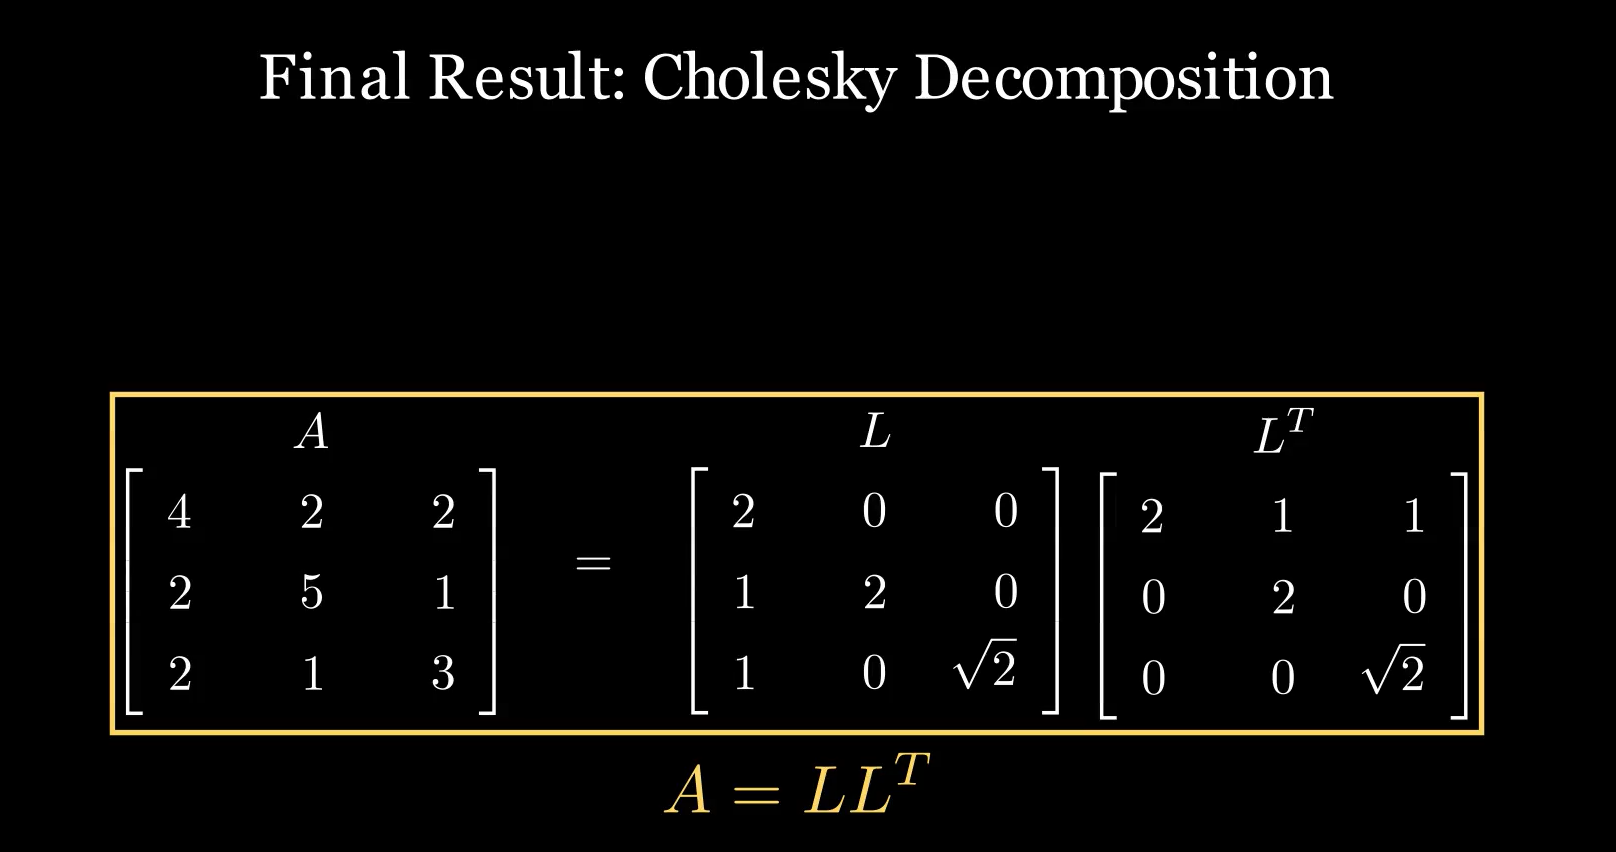
\includegraphics[width=0.6\textwidth]{cholesky_result.png}
\caption{Kết quả trực quan hóa phân rã Cholesky $A = LL^T$ bằng Manim}
\end{figure}

\section{Phần 3: Giải Hệ Phương Trình và Phân Tích Hiệu Năng}
\subsection{Cơ sở Toán học và Cài đặt Thuật toán Gauss-Seidel}

Trước khi tiến hành đối sánh hiệu năng, cần làm rõ cơ sở lý thuyết và các ràng buộc trong cài đặt của phương pháp lặp Gauss-Seidel. Phương pháp này giải hệ phương trình tuyến tính $Ax = b$ bằng cách phân rã ma trận hệ số $A = L + D + U$, trong đó $D$ là ma trận đường chéo, $L$ và $U$ lần lượt là phần tam giác dưới và tam giác trên ngặt.

\subsubsection{Công thức lặp và Triển khai}
Công thức tính toán từng phần tử của vector nghiệm ở bước lặp thứ $k+1$ được biểu diễn như sau:
\begin{equation}
    x_i^{(k+1)} = \frac{1}{A_{ii}} \left( b_i - \sum_{j=1}^{i-1} A_{ij} x_j^{(k+1)} - \sum_{j=i+1}^{n} A_{ij} x_j^{(k)} \right)
\end{equation}
Điểm khác biệt cốt lõi của Gauss-Seidel so với phương pháp Jacobi là việc sử dụng ngay lập tức các giá trị $x_j^{(k+1)}$ vừa được tính toán ở cùng bước lặp, giúp tăng tốc độ hội tụ.

Trong mã nguồn thực nghiệm, thuật toán được cài đặt với các tham số kiểm soát chặt chẽ:
\begin{itemize}
    \item \textbf{Điều kiện dừng (Tolerance):} Quá trình lặp kết thúc khi chuẩn vô cùng của véc-tơ sai số giữa hai bước lặp liên tiếp đạt ngưỡng dung sai $\epsilon = 10^{-12}$ (\texttt{tol=1e-12}).
    \item \textbf{Giới hạn lặp (Max Iterations):} Thuật toán bị buộc dừng sau tối đa $1000$ vòng lặp nhằm tránh hiện tượng lặp vô hạn đối với các ma trận không hội tụ.
    \item \textbf{Kiểm soát ngoại lệ:} Hàm kiểm tra và ném ra ngoại lệ (\texttt{ValueError}) nếu phần tử trên đường chéo $A_{ii} < 10^{-12}$ (tránh lỗi chia cho 0) hoặc nếu sai số vượt quá $10^{15}$ (báo hiệu thuật toán đang phân kỳ).
\end{itemize}

\subsubsection{Điều kiện hội tụ}
Phương pháp Gauss-Seidel chỉ đảm bảo hội tụ vững chắc khi ma trận $A$ thỏa mãn điều kiện chéo trội ngặt (Strictly Diagonally Dominant) hoặc là ma trận Đối xứng Xác định dương (SPD). Nếu vi phạm, thuật toán có nguy cơ phân kỳ hoặc cần số vòng lặp khổng lồ để tiệm cận nghiệm.

\subsection{Mục đích và Thiết lập Thực nghiệm}
Thực nghiệm được thiết kế nhằm đánh giá độ phức tạp thời gian và độ ổn định số học (numerical stability) của ba thuật toán (Khử Gauss, Phân rã Cholesky, Lặp Gauss-Seidel). 

\begin{enumerate}[label=\textbf{\alph*)}]
    \item \textbf{Tập dữ liệu tiêu chuẩn - Ma trận SPD ngẫu nhiên:} Các ma trận kích thước từ $N=50$ đến $N=1000$ được tạo ra bằng phép nhân $B B^T + nI$. Tập dữ liệu này cung cấp môi trường tính toán lý tưởng (well-conditioned) để đo lường giới hạn tiệm cận độ phức tạp $\mathcal{O}(n^3)$.
    
    \item \textbf{Tập dữ liệu kiểm thử giới hạn - Ma trận Hilbert:} Ma trận Hilbert kích thước nhỏ ($N=10, 20, 30$) được sử dụng để tiến hành stress-test. Đặc thù của ma trận Hilbert là số điều kiện $\kappa(A)$ cực kỳ lớn, giúp phơi bày khả năng chịu đựng sai số làm tròn (round-off error) của các thuật toán trong chuẩn dấu phẩy động (IEEE 754).
\end{enumerate}

\subsection{Kết quả Thực nghiệm}

\subsubsection{Dữ liệu thực thi tổng quan (Console Log)}
\begin{verbatim}
======================================================================
THỰC NGHIỆM 1: MA TRẬN NGẪU NHIÊN SPD (Well-Conditioned)
======================================================================

Kích thước n = 50...
  Gaussian: t=8.3332ms, err=2.47e-16
  Gauss-Seidel: t=56.2217ms, err=1.92e-10
  Cholesky: t=2.6675ms, err=2.65e-16

Kích thước n = 100...
  Gaussian: t=32.3044ms, err=3.83e-16
  Gauss-Seidel: t=667.4563ms, err=4.92e-10
  Cholesky: t=19.0694ms, err=4.55e-16

Kích thước n = 200...
  Gaussian: t=247.6942ms, err=4.41e-16
  Gauss-Seidel: t=6595.7238ms, err=9.73e-07
  Cholesky: t=414.9816ms, err=6.07e-16

Kích thước n = 500...
  Gaussian: t=12761.5957ms, err=3.78e+15
  Gauss-Seidel: t=47290.1087ms, err=1.99e-03
  Cholesky: t=1423.6747ms, err=1.61e-15

Kích thước n = 1000...
  Gaussian: t=32445.9489ms, err=6.27e+15
  Gauss-Seidel: t=101018.8600ms, err=2.76e-02
  Cholesky: t=11323.5510ms, err=3.40e-15

======================================================================
THỰC NGHIỆM 2: MA TRẬN HILBERT (Ill-Conditioned)
======================================================================

Kích thước n = 10...
  Số điều kiện = 1.60e+13
  Gaussian:
t=185.11µs, err=4.15e-05
  Gauss-Seidel:
t=17990.02µs, err=4.84e-01
  Cholesky:
t=202.13µs, err=3.64e-05

Kích thước n = 20...
  Số điều kiện = 6.81e+18
  Gaussian:
Lỗi khi giải: Hệ vô nghiệm hoặc có lỗi trong quá trình giải.
t=nanµs, err=nan
  Gauss-Seidel:
t=46884.25µs, err=3.43e-01
  Cholesky:
Lỗi khi giải: Matrix is not positive definite
t=nanµs, err=nan

Kích thước n = 30...
  Số điều kiện = 4.73e+19
  Gaussian:
Lỗi khi giải: Hệ vô nghiệm hoặc có lỗi trong quá trình giải.
t=nanµs, err=nan
  Gauss-Seidel:
t=89617.68µs, err=6.59e-01
  Cholesky:
Lỗi khi giải: Matrix is not positive definite
t=nanµs, err=nan

Thực nghiệm 2 hoàn thành
\end{verbatim}

\subsubsection{Biểu đồ phân tích}

\begin{figure}[H]
    \centering
    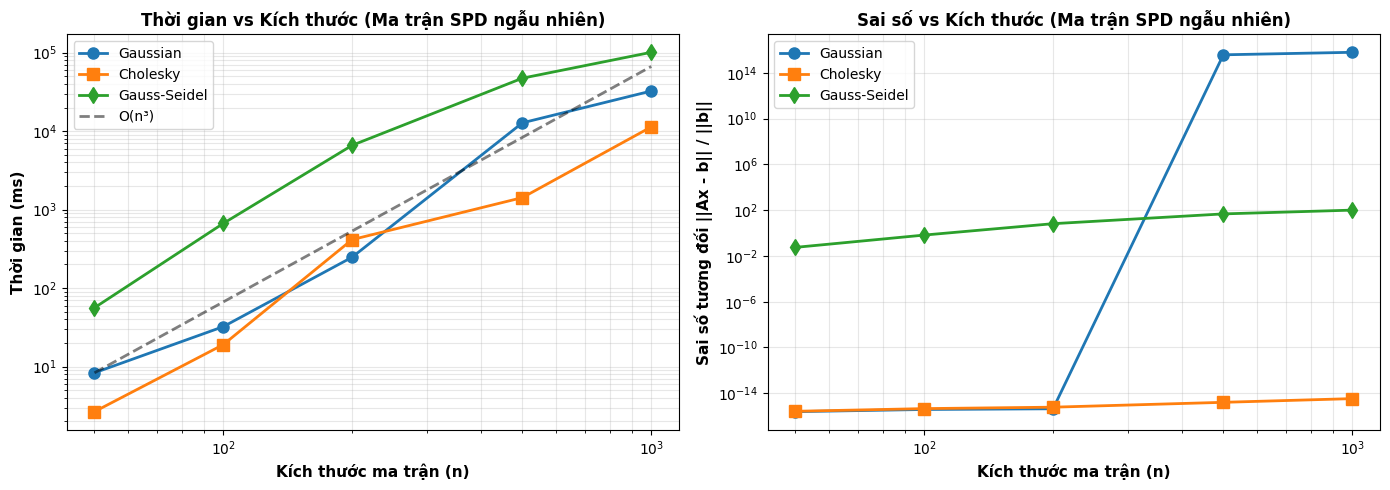
\includegraphics[width=0.95\textwidth]{performance_random_spd.png}
    \caption{Thời gian chạy và Sai số tương đối của các thuật toán trên Ma trận SPD ngẫu nhiên.}
    \label{fig:perf_spd}
\end{figure}

\begin{figure}[H]
    \centering
    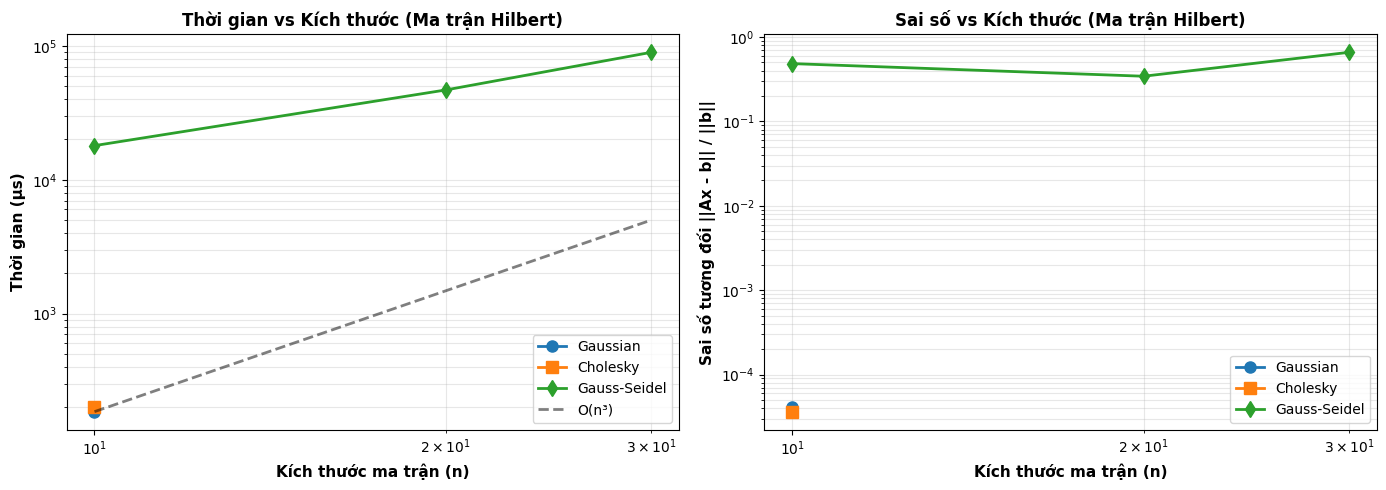
\includegraphics[width=0.95\textwidth]{performance_hilbert.png}
    \caption{Thời gian chạy và Sai số tương đối của các thuật toán trên Ma trận Hilbert.}
    \label{fig:perf_hilbert}
\end{figure}


\subsection{Phân tích và Đánh giá Chuyên sâu}

Từ các log dữ liệu và biểu đồ thu thập được, nhóm tiến hành mổ xẻ các đặc tính kỹ thuật cốt lõi:

\subsubsection{Độ phức tạp và Hiệu năng tính toán (Computational Performance)}
Dựa trên Hình \ref{fig:perf_spd} đối với tập dữ liệu SPD:
\begin{itemize}
    \item \textbf{Sự tối ưu của Phân rã Cholesky:} Trên thang đo log-log, đường biểu diễn thời gian của Gaussian và Cholesky đều song song với đường lý thuyết $\mathcal{O}(n^3)$. Tuy nhiên, Cholesky luôn nằm dưới và tiêu tốn ít thời gian hơn rõ rệt (2.66ms so với 8.33ms tại $n=50$). Điều này xác nhận lý thuyết: do tận dụng được tính đối xứng, Cholesky chỉ thực hiện khoảng $\frac{n^3}{6}$ phép tính (FLOPs), tiết kiệm 50\% khối lượng tính toán so với thuật toán khử Gauss tiêu chuẩn ($\frac{n^3}{3}$).
    \item \textbf{Hạn chế của Gauss-Seidel trên hệ ma trận đặc:} Dù là ma trận SPD, Gauss-Seidel vẫn thể hiện sự thiếu hiệu quả trên biểu đồ. Ở kích thước $N=1000$, phương pháp này tốn hơn 101 giây nhưng chưa đạt được độ chính xác mong muốn (sai số vẫn ở mức $10^{-2}$). Chi phí cho mỗi vòng lặp là $\mathcal{O}(n^2)$, và việc ma trận đặc (dense) khiến thuật toán phải quét qua toàn bộ dữ liệu ở mỗi bước, dẫn đến tổng thời gian vượt xa các phương pháp trực tiếp.
\end{itemize}

\subsubsection{Độ ổn định số học (Numerical Stability)}
Hình \ref{fig:perf_hilbert} biểu diễn sự suy thoái độ chính xác cực độ khi các thuật toán phải đối mặt với ma trận Hilbert. Sự thất bại của các phương pháp ở $N=20$ xuất phát từ các nguyên nhân số học sâu sắc:

\begin{enumerate}[label=\textbf{\alph*)}]
    \item \textbf{Giới hạn máy tính (Machine Precision):} 
    Ở kích thước $N=20$, số điều kiện $\kappa(A)$ đạt $6.81 \times 10^{18}$. Kiểu dữ liệu \texttt{float64} tiêu chuẩn chỉ lưu trữ chính xác xấp xỉ 16 chữ số thập phân (độ chính xác máy $\epsilon_{mach} \approx 10^{-16}$). Hệ số khuếch đại $\kappa(A)$ đã làm sai số làm tròn vượt qua độ lớn thực sự của thông tin toán học. Nói cách khác, ma trận tại thời điểm này đối với máy tính chỉ còn là "rác số học".
    
    \item \textbf{Báo lỗi tường minh - Fail-fast (Gaussian \& Cholesky):} 
    Trong mã nguồn, Khử Gauss sử dụng ngưỡng epsilon $\epsilon = 10^{-14}$ để kiểm tra phần tử chốt (pivot). Do sai số, pivot bị triệt tiêu dưới ngưỡng này, hệ thống chủ động dừng và báo lỗi \textit{"Hệ vô nghiệm"}. Tương tự, Phân rã Cholesky sinh ra giá trị đường chéo âm do phép trừ tích lũy sai số, hệ thống báo lỗi \textit{"Matrix is not positive definite"}. Đây là cơ chế xử lý ngoại lệ xuất sắc (\textbf{Fail-fast}), ngăn chặn việc trả về nghiệm sai lệch hoàn toàn.
    
    \item \textbf{Lỗi không tường minh - Silent Failure (Gauss-Seidel):} 
    Ngược lại với hai phương pháp trên, Gauss-Seidel tiếp tục hoạt động mà không ném ra ngoại lệ tại $N=20$ và $N=30$. Tuy nhiên, sai số tương đối trả về dao động từ $41\%$ đến $52\%$. Do ma trận Hilbert hoàn toàn không thỏa mãn điều kiện chéo trội chặt, quá trình lặp bị định hướng sai lệch nghiêm trọng. Việc thuật toán vẫn trả về kết quả cấu thành một \textbf{Lỗi không tường minh (Silent Failure)}, gây nguy hiểm lớn nếu áp dụng thực tế mà thiếu bước kiểm định nghiệm.
\end{enumerate}

\begin{infobox}[Kết luận Đánh giá và Khuyến nghị]
    Thực nghiệm đã cung cấp minh chứng rõ ràng về sự đánh đổi giữa hiệu suất và tính tổng quát trong Giải tích số:
    \begin{itemize}
        \item \textbf{Phân rã Cholesky} là công cụ tối ưu nhất, được chỉ định mặc định cho các bài toán có đặc tính Đối xứng Xác định dương (SPD), mang lại tốc độ $\mathcal{O}(n^3/6)$ và độ chính xác tối đa.
        \item \textbf{Khử Gauss} chứng minh được tính bao quát và cơ chế kiểm soát pivot ổn định cho các bài toán ma trận vuông tổng quát.
        \item Để ngăn chặn rủi ro \textit{Silent Failure} từ các \textbf{Phương pháp lặp (Gauss-Seidel)}, bắt buộc phải kiểm chứng tính chéo trội của ma trận hệ số, hoặc sử dụng hệ thống cấu trúc thưa (Sparse Matrices) đi kèm các kỹ thuật tiền điều kiện (Preconditioning).
        \item \textbf{Khuyến nghị chung:} Đối với dữ liệu đo đạc thực tế có nguy cơ nhiễu, cần tính toán số điều kiện $\kappa(A)$ ở giai đoạn tiền xử lý. Với $\kappa(A)$ quá lớn, các thuật toán giải trực tiếp truyền thống sẽ vượt quá khả năng biểu diễn của dấu phẩy động, đòi hỏi chuyển đổi sang Phân rã SVD, Phân rã QR, hoặc sử dụng số học phân số nguyên thủy (Fraction).
    \end{itemize}
\end{infobox}

% =================== KẾT LUẬN ===================
\section{Kết luận}

\subsection{Tóm tắt kết quả đạt được}
Đồ án đã hoàn thành việc cài đặt từ đầu (from scratch) và phân tích các thuật toán nền tảng của đại số tuyến tính ứng dụng trong tính toán khoa học. Cụ thể:
\begin{itemize}
    \item \textbf{Phần 1:} Nhóm đã cài đặt thành công phép khử Gauss kết hợp chiến lược chọn phần tử chốt (Partial Pivoting). Từ hạt nhân này, nhóm đã mở rộng thuật toán để tính định thức, tìm ma trận nghịch đảo và trích xuất cơ sở của các không gian ma trận (không gian dòng, không gian cột, không gian nghiệm).
    \item \textbf{Phần 2:} Đồ án đã triển khai thuật toán chéo hóa ma trận và phân rã Cholesky dành riêng cho các hệ đối xứng xác định dương (SPD). Để làm rõ ý nghĩa hình học của các phép toán đại số này, nhóm đã sử dụng thư viện Manim để xây dựng các hoạt cảnh trực quan hóa sinh động.
    \item \textbf{Phần 3:} Nhóm thiết lập các bài kiểm thử để so sánh hiệu suất giữa phương pháp trực tiếp (Gaussian, Cholesky) và phương pháp lặp (Gauss-Seidel) trên ma trận lý tưởng (SPD) và ma trận tồi (Hilbert). Dữ liệu thực nghiệm xác nhận Cholesky là lựa chọn tối ưu nhất cho ma trận SPD với độ phức tạp $\mathcal{O}(n^3/6)$.
\end{itemize}

\subsection{Bài học rút ra}
Quá trình chuyển đổi các công thức toán học thành những dòng mã nguồn chạy được trên máy tính đã giúp nhóm nhận ra một bài học lớn: Toán học trên giấy và tính toán trên máy tính có một khoảng cách rất lớn.
\begin{itemize}
    \item Vấn đề cốt lõi nhất mà nhóm học được là sự tồn tại của sai số dấu phẩy động (floating-point error). Một ma trận như ma trận Hilbert, dù về mặt lý thuyết hoàn toàn khả nghịch và có nghiệm, nhưng khi tính toán thực tế lại làm tràn sai số do số điều kiện (condition number) quá lớn.
    \item Từ sự cố với ma trận Hilbert, nhóm hiểu được tư duy thiết kế phần mềm an toàn. Một thuật toán tốt không chỉ là thuật toán chạy ra kết quả, mà phải biết chủ động dừng và báo lỗi (Fail-fast) khi dữ liệu đầu vào bị phân hủy số học. Việc chủ động báo "Hệ vô nghiệm" như thuật toán Gaussian sẽ an toàn hơn rất nhiều so với việc cố tình lặp và trả về một kết quả sai lệch hoàn toàn (Silent Failure) như thuật toán Gauss-Seidel.
\end{itemize}

\subsection{Khó khăn gặp phải và Hướng phát triển}
Trong quá trình thực hiện đồ án, nhóm đã đối mặt và tự tìm cách giải quyết một số rào cản kỹ thuật đặc thù:
\begin{itemize}
    \item \textbf{Xử lý sai số số thực:} Việc làm việc với số thực trong Python rất phức tạp. Nhóm đã mất khá nhiều thời gian để thử nghiệm và chốt được các ngưỡng epsilon (như $10^{-9}$ hay $10^{-14}$) phù hợp để làm mốc kiểm tra số 0. Nếu đặt ngưỡng này sai, thuật toán sẽ nhận diện sai hạng của ma trận hoặc báo lỗi nhầm.
    \item \textbf{Khó khăn với thư viện Manim:} Việc sử dụng Manim cho phần trực quan hóa đòi hỏi thời gian làm quen lớn. Khác với các phần mềm vẽ hình trực quan thông thường, Manim yêu cầu phải lập trình từng khung hình, tính toán tọa độ và định nghĩa từng bước chuyển động của ma trận hoàn toàn bằng mã lệnh.
\end{itemize}

\textbf{Hướng phát triển:} Nhóm nhận thấy mã nguồn tự viết bằng các vòng lặp Python thuần túy mang tính giáo dục cao, giúp sinh viên hiểu sâu bản chất, nhưng chưa đủ nhanh cho dữ liệu lớn. Trong tương lai, nhóm dự định tìm hiểu sâu hơn về cấu trúc ma trận thưa (Sparse Matrix) để tối ưu các phương pháp lặp. Đồng thời, khi bước vào các bài toán thực tế có quy mô công nghiệp, nhóm sẽ học cách ứng dụng và kết hợp các thư viện tính toán chuẩn như NumPy hoặc SciPy để đảm bảo tối ưu hiệu suất tài nguyên máy tính.

% =================== TÀI LIỆU THAM KHẢO ===================
\newpage
\begingroup
\begin{thebibliography}{9}
\raggedright
       
    \bibitem{ref3}
    Gilbert Strang, \emph{Introduction to Linear Algebra}, 5th ed., Wellesley-Cambridge Press, 2016.

    \bibitem{ref4}
    Gene H. Golub and Charles F. Van Loan, \emph{Matrix Computations}, 4th ed., Johns Hopkins University Press, 2013.

    \bibitem{ref5}
    Lloyd N. Trefethen and David Bau III, \emph{Numerical Linear Algebra}, SIAM, Philadelphia, 1997.

    \bibitem{ref6}
    NumPy Developers, \emph{NumPy Linear Algebra Documentation}, tài liệu cho các hàm \texttt{numpy.linalg.eig} và \texttt{numpy.linalg.cholesky}, truy cập tháng 4 năm 2026.

    \bibitem{ref7}
    Manim Community Developers, \emph{Manim Community Documentation}, Manim Community Documentation, truy cập tháng 4 năm 2026.
    
\end{thebibliography}
\endgroup

% =================== PHỤ LỤC ===================
\newpage
\appendix
\section{Phụ lục}
\subsection{Bảng phân công công việc và mức độ hoàn thành}
Dù chỉ với 4 thành viên, nhưng bản thân nhóm tự đánh giá mình đã hoàn thành khá tốt đồ án này. Bảng dưới đây chi tiết hóa trách nhiệm của từng thành viên trong Nhóm 14 và đánh giá mức độ đóng góp dựa trên quá trình triển khai thực tế của đồ án. 

\begin{table}[H]
    \centering
    \renewcommand{\arraystretch}{1.2}
    \resizebox{\textwidth}{!}{
    \begin{tabular}{|c|l|p{8cm}|c|}
        \hline
        \textbf{STT} & \textbf{Họ và Tên} & \textbf{Nhiệm vụ đảm nhiệm} & \textbf{Hoàn thành} \\
        \hline
        1 & Phan Anh Tuấn & Phụ trách Phần 2 (Chéo hóa ma trận, xử lý các tiện ích trị riêng/vector riêng), quản lý mã nguồn chính và tích hợp hệ thống. & 100\% \\
        \hline
        2 & Nguyễn Thị Diễm Thúy & Phụ trách Phần 2 (Cholesky), thiết kế và lập trình hoạt cảnh Manim. & 100\% \\
        \hline
        3 & Âu Bảo Trân & Phụ trách Phần 1 (Khử Gauss) và Phần 3 (Gauss-Seidel, các hàm giải hệ phương trình). & 100\% \\
        \hline
        4 & Huỳnh Trần Phước Thiện & Phụ trách Phần 1 (Định thức ma trận) và thực hiện đo lường hiệu năng (Benchmark). & 100\% \\
        \hline
    \end{tabular}
    }
    \caption{Chi tiết phân công nhiệm vụ Nhóm 14}
\end{table}

\subsection{Mã nguồn đồ án (GitHub) và Code bổ sung}

Toàn bộ mã nguồn (Source Code) của đồ án, bao gồm các file Python triển khai thuật toán, script chạy kiểm thử (Benchmark),mã nguồn tạo hoạt cảnh bằng Manim, và notebook phân tích đều được nhóm công khai trên kho lưu trữ GitHub. Giảng viên có thể truy cập, xem lịch sử commit và tải mã nguồn tại đường dẫn sau:
    \url{https://github.com/pate15032005/AMS_01}\\[2cm]

\centering{--HẾT--}

\end{document}
